%Simon Krenger: Diskrete Mathematik
\documentclass{report}
\usepackage{amsmath}
\usepackage{amsthm}
\usepackage{amssymb}
\usepackage[utf8]{inputenc} 
\usepackage{graphicx}

\newtheorem{mydef}{Definition}
\newtheorem{myexample}{Beispiel}
\newtheorem{myproof}{Beweis}
\newtheorem{axiom}{Axiom}

\title{Diskrete Mathematik}
\author{Simon Krenger, Christian Meyer}

\begin{document}
\maketitle
\chapter{Logik (Boolesche Algebra)}
Nach George Bool, 1815 bis 1864, Cork (Irland)
\section{Aussagen}
Wir betrachten Aussagen (Sätze), die entweder wahr (1) oder falsch (0) sind.

\begin{quote}Heute ist Freitag \(\to\) wahr\end{quote}
\begin{quote}Morgen schneit es in Bern \(\to\) falsch\end{quote}
\begin{quote}Schauen Sie einmal! \(\to\) keine Aussage\end{quote}
Aussagen bezeichnen wir mit a, b, c, d, …
\begin{mydef}
Ist a eine Aussage, somit heisst  \(\lnot\)a die \underline{Negation} von a
\end{mydef}

\section{Konjunktion}
Wir verbinden zwei Aussagen a, b mit Hilfe von “und” zu einer einzigen Aussage
\begin{equation}a \land b\end{equation}

Die Wahrheitstabelle von a \(\land\) b sind abhängig von denjenigen von a als auch von b. Dies stellen wir in einer \underline{Wahrheitswerttabelle} dar. Wir finden sofort die Regeln
\begin{equation}a \land \lnot a = falsch\end{equation}


\begin{mydef}Eine Aussage, die immer falsch ist, heisst \underline{Kontradiktion}.\end{mydef}

\begin{equation}a \land 1 = a\end{equation}
\begin{equation}a \land 0 = 0\end{equation}
Weiter finden wir Gesetze
\begin{quote}Kommutativgesetz (Vertauschungsgesetz)\end{quote}
\begin{equation}a \land b = b \land a\end{equation}
\begin{myproof}Wir beweisen mit einer Wahrheitswerttabelle
\begin{center}\begin{tabular}{c c | c c}
a & b & a \(\land\) b & b \(\land\) a\\
\hline
0 & 0 & 0 & 0  \\
0 & 1 & 0 & 0  \\
1 & 0 & 0 & 0 \\
1 & 1 & 1 & 1 \\
\end{tabular}\end{center}\end{myproof}
\begin{quote}Assoziativgesetz (Verbindungsgesetz)\end{quote}
\begin{equation}a \land (b \land c) = (a \land b) \land c\end{equation}
\begin{myproof}Wir beweisen mit einer Wahrheitswerttabelle
\begin{center}\begin{tabular}{c c c | c c}
a & b & c & a \(\land\) (b \(\land\) c) & (a \(\land\) b) \(\land\) c\\
\hline
0 & 0 & 0 & 0 & 0  \\
0 & 0 & 1 & 0 & 0  \\
0 & 1 & 0 & 0 & 0 \\
0 & 1 & 1 & 0 & 0 \\
1 & 0 & 0 & 0 & 0 \\
1 & 0 & 1 & 0 & 0 \\
1 & 1 & 0 & 0 & 0 \\
1 & 1 & 1 & 1 & 1 \\
\end{tabular}\end{center}\end{myproof}
\begin{quote}Idempotenzgesetz\end{quote}
\begin{equation}a \land a = a\end{equation}
\section{Disjunktion}
Zwei Aussagen a, b werden mit der Disjunktion "oder" zu einer neuen Aussage verbunden. Dafür schreiben wir:\begin{equation}a \lor b\end{equation}
und definieren
\begin{center}\begin{tabular}{c c | c}
a & b & a \(\lor\) b\\
\hline
0 & 0 & 0  \\
0 & 1 & 1  \\
1 & 0 & 1 \\
1 & 1 & 1 \\
\end{tabular}\end{center}
Nicht verwechseln mit "entweder oder" (XOR)! Wir finden die Regeln
\begin{equation}a \lor 1 = 1\end{equation}
\begin{equation}a \lor 0 = a\end{equation}
\begin{equation}a \lor \lnot a = 1\end{equation}
\begin{mydef}Eine Aussage, die stets wahr ist, heisst \underline{Tautologie}.\end{mydef}
Es gelten die Gesetze
\begin{quote}Kommutativgesetz\end{quote}
\begin{equation}a \lor b = b \lor a\end{equation}
\begin{quote}Assoziativgesetz\end{quote}
\begin{equation}a \lor (b \lor c) = (a \lor b) \lor c\end{equation}
\begin{quote}Idempotenzgesetz\end{quote}
\begin{equation}a \lor a = a\end{equation}
In der Algebra in \(\mathbb{R}\) gilt
\begin{equation}a(b+c) = ab+ac\end{equation}
was in der Logik zu
\begin{equation} \label{eq:distributivgesetz}a \land (b \lor c) = (a \land b) \lor (a \land c)\end{equation}
\begin{equation}a \lor (b \land c) = (a \lor b) \land (a \lor c)\end{equation}
dem \underline{Distributivgesetz} (Verteilungsgesetz) führt. Der folgende Beweis zeigt, dass die Gleichung \ref{eq:distributivgesetz} gilt.
\begin{myproof}Wir beweisen mit einer Wahrheitswerttabelle
\begin{center}\begin{tabular}{c c c | c c c c c}
a & b & c & b \(\lor\) c & a \(\land\) (b \(\lor\) c) & a \(\land\) b & a \(\land\) c & (a \(\land\) b) \(\lor\) (a \(\land\) c)  \\
\hline
0 & 0 & 0 & 0 & 0 & 0 & 0 & 0  \\
0 & 0 & 1 & 1 & 0 & 0 & 0 & 0  \\
0 & 1 & 0 & 1 & 0 & 0 & 0 & 0 \\
0 & 1 & 1 & 1 & 0 & 0 & 0 & 0 \\
1 & 0 & 0 & 0 & 0 & 0 & 0 & 0 \\
1 & 0 & 1 & 1 & 1 & 0 & 1 & 1 \\
1 & 1 & 0 & 1 & 1 & 1 & 0 & 1 \\
1 & 1 & 1 & 1 & 1 & 1 & 1 & 1 \\
\end{tabular}\end{center}
Das zweite Distributivgesetz kann analog dazu bewiesen werden.\end{myproof}
In der Logik gibt es zu jedem Gesetz ein \underline{duales Gesetz}. Dies entsteht durch wechseln von \(\lor\) zu \(\land\) und umgekehrt. Weiter finden wir
\begin{quote}Absorbtionsgesetz\end{quote}
\begin{equation}a \land (a \lor b) = a\end{equation}
\begin{equation}a \lor (a \land b) = a\end{equation}
\begin{myproof}Wir beweisen mit einer Wahrheitswerttabelle
\begin{center}\begin{tabular}{c c | c c}
a & b & a \(\lor\) b & a \(\land\) (a \(\lor\) b) \\
\hline
0 & 0 & 0 & 0  \\
0 & 1 & 1 & 0  \\
1 & 0 & 1 & 1  \\
1 & 1 & 1 & 1 \\
\end{tabular}\end{center}\end{myproof}
\begin{quote}Gesetz von de Morgan\end{quote}
\begin{equation}\lnot (a \land b) = \lnot a \lor \lnot b\end{equation}
\begin{equation}\lnot (a \lor b) = \lnot a \land \lnot b\end{equation}
Wir verwenden die Gesetze, um die Aussagen zu vereinfachen.

\section{Implikation}
Mathematische Lehrsätze haben die Form "Wenn ein Dreieck rechtwinklig ist mit Hypothenuse $c$ und Katheten $a$, $b$, dann ist $c^2=a^2+b^2$"\\
Sie bestehen also aus Voraussetzung(en):
\begin{quote}Das Dreieck ist rechtwinklig\end{quote}
und Behauptung
\begin{quote}Es ist $a^2+b^2=c^2$\end{quote}
und einem Beweis
\begin{myproof}Gemäss "Indischer Beweis":
\begin{eqnarray}c^2&=&4\frac{ab}{2}+(a-b)^2 \nonumber \\
c^2&=&2ab+a^2-2ab+b^2\nonumber \\
c^2&=&a^2+b^2\end{eqnarray}\end{myproof}
Im obrigen Beispiel haben wir einen direkten Beweis geführt. Von der Voraussetzung durch Rechnung zur Behauptung.\\
Wenn wir zwei Aussagen a, b mit "wenn a, dann b" oder "wenn a so b" oder "aus a folgt b (a impliziert b)" verknüpfen, so schreiben wir dafür
\begin{equation}a \to b\end{equation}
und definieren
\begin{center}\begin{tabular}{c c | c}
a & b & a \(\to\) b\\
\hline
0 & 0 & 1  \\
0 & 1 & 1  \\
1 & 0 & 0 \\
1 & 1 & 1 \\
\end{tabular}\end{center}
Wir finden sofort, das "aus a folgt b"
\begin{equation}a \to b = \lnot a \lor b\end{equation}

Wollen wir zeigen, dass ein Satz falsch ist, so genügt ein einziges Beispiel, dass wir \underline{Gegenbeispiel} nennen, um die Behauptung zu widerlegen.\\

\subsection{Umkehrung, Kontraposition}
\begin{mydef}Hat eine Aussage die Form
\begin{equation}a \to b\end{equation}
so heisst
\begin{equation}b \to a\end{equation}
die \underline{Umkehrung}.
\end{mydef}
Ist eine Aussage, ein Satz wahr, so muss die Umkehrung nicht wahr sein, wie zum Beispiel:
\begin{quote}"Wenn ich Geburtstag habe, so esse ich einen Kuchen"\end{quote}
\begin{quote}"Wenn ein Mensch glücklich ist, so trinkt er Sinalco"\end{quote}
Wir finden aber, dass
\begin{eqnarray}\lnot b \to \lnot a = \lnot(\lnot b) \lor \lnot a \nonumber\\
= b \lor \lnot a = \lnot a \lor b = a \to b\end{eqnarray}
\begin{mydef}Wir nennen
\begin{equation}\lnot b \to \lnot a\end{equation}
die \underline{Kontraposition} von
\begin{equation}a \to b\end{equation}
\end{mydef}
Wir haben gezeigt, dass $\lnot b \to \lnot a = a \to b$ ist, was bedeutet, dass bei einem wahren Satz auch dessen Kontraposition wahr ist.
\begin{quote}{Satz}: "Wenn es heute Freitag ist, so gehe ich ein Bier trinken."\end{quote}
\begin{quote}{Kontraposition}: "Wenn ich nicht ein Bier trinken gehe, so ist heute Freitag"\end{quote}
Manchmal ist der direkte Beweis eines Satzes zu schwierig oder nicht möglich, dann beweisen wir die Kontraposition.
\begin{quote}{Satz}: Ist $n \in \mathbb{N}$ und $n^2$ eine gerade Zahl, so ist $n$ auch eine gerade Zahl.\end{quote}
\begin{myproof}Der direkte Beweis
\begin{eqnarray}n^2 &=& 2p \land p \in \mathbb{N} \nonumber \\
\to n &=& \sqrt{2} \cdot \sqrt{p}\end{eqnarray}
gelingt nicht. Grund dafür ist, dass eine irrationale Zahl ($\sqrt{2}$) per Definition ein nichtperiodischer, nichtendlicher Dezimalbruch ist.\end{myproof}
Also beweisen wir die Kontraposition:
\begin{quote}{Kontraposition}: "Ist $n \in \mathbb{N}$ und $n$ ungerade, so ist auch $n^2$ ungerade"\end{quote}
\begin{myproof}\begin{eqnarray} 
n &=& 2p + 1 \quad \land p \in \mathbb{N}_0 \nonumber \\
\to n^2 &=& (2p + 1)^2 \nonumber \\
n^2 &=& 4p^2 + 4p + 1 \nonumber \\
n^2 &=& 2 (2p^2 + 2p) + 1\label{eq:nungerade} \end{eqnarray}
Also ist $n^2$ eine ungerade Zahl.\qed\end{myproof}

\section{Aequivalenz}
Wenn zwei Aussagen gleichwertig (aequivalent) sind, wenn also
\begin{equation}(a \to b) \land (b \to a)\end{equation}
so schreiben wir dafür
\begin{equation}a \iff b\end{equation}
und finden die Wahrheitswerte
\begin{center}\begin{tabular}{c c | c}
a & b & a \(\iff\) b\\
\hline
0 & 0 & 1 \\
0 & 1 & 0 \\
1 & 0 & 0 \\
1 & 1 & 1 \\
\end{tabular}\end{center}
Wir finden die Umformung
\begin{eqnarray}
a \iff b &=& (a \to b) \land (b \to a)\nonumber \\
&=& (\lnot a \lor b) \land (\lnot b \lor a)\nonumber \\
&=& (\lnot a \land b) \lor (\lnot a \land a) \lor (b \land \lnot b) \lor (a \land b) \nonumber \\
&=& (a \land b) \lor (\lnot a \land \lnot b)
\end{eqnarray}
Ausserdem ist 
\begin{equation}a \iff b = \lnot (a \veebar b)\end{equation}
also
\begin{eqnarray}a \veebar b &=& [(a \land b) \lor (\lnot a \land \lnot b)] \nonumber \\
&=&\lnot(a \land b) \land \lnot (\lnot a \land \lnot b) \nonumber \\
&=&(\lnot a \lor \lnot b) \land (a \lor b)\end{eqnarray}
Wenn wir in der Mathematik einen Satz finden, dessen Umkehrung auch wahr ist, so wählen wir die Formulierung mit
\begin{quote}"dann und nur dann" oder "genau dann"\end{quote}
im Englischen
\begin{quote}"if and only if" oder "iff"\end{quote}

Manchmal gelingt es nicht, die linke Seite in die rechte Seite umzuformen. Dann verwenden wir die Eigenschaft
\begin{quote}"Wenn $l=x$ und $r=x$, so ist $l=r$\end{quote}
Wir formen also die linke Seite zuerst einmal um und dann \underline{unabhängig davon} die rechte Seite und hoffen, dass wir beide Male das gleiche Resultat ($x$) erhalten.\\\\
Genau gleich behandeln wir Behauptungen der Logik wenn es um die Aequivalenz zweier Aussagen geht.

\section{Logische Schlüsse}
Wir gehen aus von verschiedenen \underline{Prämissen} wie
\begin{eqnarray}\mbox{Prämisse 1} & & p_1 = a \land b \nonumber \\
\mbox{Prämisse 2}& & p_2 = \lnot a \nonumber \\
\mbox{Prämisse 3}& & p_3 = a \land \lnot b\end{eqnarray}
und ziehen daraus eine \underline{Konklusion} $k : a \lor b$. Nun fragen wir uns, ob die Konklusion bei diesen Prämissen richtig ist. Ist dies der Fall, so sprechen wir von einem logischen Schluss (wenn also das die richtige Konklusion ist).
\\\\Es muss also
\begin{equation}(p_1 \land p_2 \land ... \land p_n) \to k = 1\end{equation}
eine Tautologie sein. Im Beispiel ist also
\begin{equation}[(a \land b) \land \lnot a \land (a \land \lnot b)] \to (a \lor b)\end{equation}
so lange umgeformt werden, bis erkenntlich ist, ob eine Tautologie vorliegt oder nicht.
\begin{eqnarray}& &[(a \land b) \land \lnot a \land (a \land \lnot b)] \to (a \lor b) \nonumber \\
&=&(a \land b \land \lnot a \land a \land \lnot b) \to (a \lor b) \nonumber \\
&=&0 \to (a \lor b) \nonumber \\
&=&\lnot 0 \lor (a \lor b) = 1 \lor (a \lor b) = 1\end{eqnarray}
und damit liegt ein logischer Schluss vor.\\\\
In der Logik schreiben wir Prämissen und Konklusion untereinander wie zum Beispiel
\begin{equation}\frac{a \to b \quad\quad a \land b \to c \quad\quad c}{a}\end{equation}

Verschiedene bekannte logische Schlüsse besitzen einen Namen, wie zum Beispiel die Folgdenden:
\begin{enumerate}
\item \underline{modus ponens} (Abtrennungsregel)
\begin{equation}\frac{a \to b \quad\quad a}{b}\end{equation}
ist ein logischer Schluss, denn
\begin{eqnarray}& &[(a \to b) \land a] \to b \nonumber \\
&=&[(\lnot a \lor b) \land a] \to b \nonumber \\
&=&(a \land b) \to b \nonumber \\
&=&\lnot (a \land b) \lor b \nonumber \\
&=&\lnot a \lor \lnot b \lor b = \lnot a \lor 1 = 1\end{eqnarray}
Es ist die Art und Weise, wie wir einen mathematischen Satz $a \to b$ anwenden.
\item \underline{modus tollens} (Aufhebende Schlussweise)
\begin{equation}\frac{a \to b \quad\quad \lnot b}{\lnot a}\end{equation}
ist ein logischer Schluss, denn
\begin{eqnarray}& &[(a \to b) \land \lnot b] \to \lnot a \nonumber \\
&=&[(\lnot a \lor b) \land \lnot b] \to \lnot a \nonumber \\
&=&[(b \land \lnot b) \lor (\lnot a \land \lnot b)] \to \lnot a \nonumber \\
&=&(\lnot a \land \lnot b) \to \lnot a \nonumber \\
&=&\lnot (\lnot a \land \lnot b) \lor \lnot a \nonumber \\
&=&a \lor b \lor \lnot a = 1 \lor b = 1\end{eqnarray}
\item \underline{reductio ad absurdum} (zurückführen auf einen Widerspruch)
\begin{equation} \frac{a \to (b \land \lnot b)}{\lnot a}\end{equation}
ist ein logischer Schluss, denn
\begin{eqnarray}& &[a \to (b \land \lnot b)] \to \lnot a \nonumber \\
&=&[a \to 0] \to \lnot a \nonumber \\
&=&[\lnot a \lor 0] \to \lnot a \nonumber \\
&=&\lnot a \to \lnot a = a \lor \lnot a = 1\end{eqnarray}
Dieser logische Schluss führt uns zum \underline{Beweis mit Gegenannahme}.\\\\
Wollen wir beweisen, dass ein Satz $s$ wahr ist und gelingt uns dies nicht mit einem direkten Beweis oder mit einem Beweis mit Kontraposition, so wählen wir die Gegenannahme:
\begin{quote}$\lnot s$ ist wahr\end{quote}
und zeigen, dass dies zu einem Widerspruch führt wie $\lnot b \land b$ oder $1 = 2$ oder ähnlich.\\\\
Dann sagt uns die "reductio ad absurdum", dass meine Gegenannahme falsch ist und damit die Aussage $s$ wahr ist.\end{enumerate}
Einen Beweis mit Gegenannahme nennen wir auch einen \underline{indirekten Beweis}. Dieses Beweisverfahren können wir auch für logische Schlüsse anwenden.\\\\
Ist
\begin{equation}\frac{a \land \lnot b \quad a \to b}{a \lor b}\end{equation}
ein logischer Schluss?
\begin{quote}Gegenannahme: Es ist liegt kein logischer Schluss vor und damit ist
\begin{equation}[(a \land \lnot b) \land (a \to b)] \to (a \lor b) = 0\end{equation}\end{quote}
Nun zeigen wir, dass die Gegenannahme zu einem Widerspruch führt. Wir haben die Aussage
\begin{equation}x \to y = 0 \nonumber\end{equation}
Also muss $x=1$ und $y=0$ sein.\\\\
Es ist $x = p_1 \land p_2 \land ... \land p_n$ (Alle Prämissen und damit muss auch
\begin{equation}p_1 = p_2 = ... = p_n = 1 \nonumber \end{equation}
sein. Um den Widerspruch zu sehen, machen wir eine Tabelle:
\begin{equation}\begin{tabular}{c | c | c | c | c |}
& $a \land \lnot b$ & $a \to b$ & $\to$ & $a \lor b$ \\ \hline
1) & \underline{1} & 1 & & 0 \\ \hline
2) & & & & $a=0, b=0$ \\ \hline
3) &\underline{$0 \land 1 = 0$} & & & \\ \hline
\end{tabular}\end{equation}Bei den unterstrichenen Werten haben wir einen Widerspruch hergeführt. Die Gegenannahme ist falsch, also liegt ein logischer Schluss vor.

\section{Prädikatenlogik}
Einige Aussagen wie
\begin{itemize}
\item Informatiker(innen) besitzen einen Laptop
\item Katzen schnurren
\item Hunde bellen
\item $a \cdot b = b \cdot a$\end{itemize}
verlangen eine Präzisierung wie
\begin{itemize}
\item Nicht alle Informatiker(innen) besitzen einen Laptop
\item Einige Katzen schnurren
\item Alle Hunde bellen
\item Für alle $a,b \in \mathbb{R}$ ist $a \cdot b = b \cdot a$\end{itemize}
WIr brauchen also ein \underline{Prädikat} (Aussage) über Grössen aus einer bestimmten \underline{Menge} und einen \underline{Quantor}.
Wir nennen $\forall$ den \underline{Allquantor}. Damit bedeutet
\begin{quote}$x \in M: \forall x (P(x))$\\
(Für alle $x$ gilt $P(x)$")\end{quote}
dass alle Elemente der Menge $M$ das Prädikat $P$ besitzen.\\\\
Wählen wir
\begin{quote}$M = \{s \quad|\quad s \quad$ ist Student(in)$\}$ \\
$q(s): s$ ist in der Klasse I1q\end{quote}
so können wir formulieren
\begin{equation}s \in M : \forall s (q(s))\end{equation}
was natürlich falsch ist. Korrekt ist
\begin{equation}\lnot \forall s (q(s)) \quad \mbox{oder auch} \quad \not \forall s(q(s))\end{equation}
geschrieben. Dieses "nicht alle" ist gleichbedeutend mit
\begin{quote}"Es gibt (mindestens) ein(e)"\end{quote}
was wir mit dem \underline{Existenzquantor $\exists$} so schreiben:
\begin{equation}\exists s(\lnot q(s))\end{equation}
Wir haben also
\begin{equation}\lnot \forall x (P(x)) = \exists x ( \lnot P(x))\end{equation}
Betrachten wir
\begin{quote}$K = \{k\quad|\quad k \quad  $Ist eine Katze$\}$\\
$s(k) : k$ schnurrt\end{quote}
und
\begin{equation}k \in K : \exists k (s(k))\end{equation}
was "es gibt mindestens eine Katze, die schnurrt" bedeutet. Verneinen wir die Aussage
\begin{equation}\lnot \exists k (s(k)) \quad \mbox{oder} \quad \not \exists k (s(k))\end{equation}
so bedeutet dies: "Es gibt keine Katze, die schnurrt.", was gleichbedeutend ist mit "Alle Katzen schnurren nicht", also
\begin{equation}\lnot \exists k (s(k)) = \forall k (\lnot s(k))\end{equation}
Auch in der Mathematik werden die Quantoren verwendet wie zum Beispiel
\begin{enumerate}
\item \begin{equation}a,b \in \mathbb{R} : \forall a \forall b (ab = ba)\end{equation}
oder auch\begin{equation}a,b \in \mathbb{R} : \forall a,b (ab = ba)\end{equation}
\item \begin{equation}a \in \mathbb{R} \backslash \{0\}, x \in \mathbb{R}: \forall a \exists x (ax=1)\end{equation} Wir nennen $x=a^{-1}$ das zu $a$ \underline{inverse Element}.
\end{enumerate}
\subsection{Zwei Prädikate}
Oft ist es einfacher, wenn eine Aussage mit Hilfe von zwei Prädikaten formuliert wird. Für
\begin{quote}"Alle Informatik-Studierenden besitzen ein iPhone"\end{quote}
wählen wir
\begin{quote}$s = \{s \quad | \quad s \quad$ ist Student(in)$\}$ \\
$i(s) : s$ studiert Informatik\\
$p(s): s$ besitzt ein iPhone\end{quote}
und schreiben
\begin{equation}s \in S: \forall s (i(s) \to p(s))\end{equation}
ist die Aussage falsch, weil nicht alle Informatik-Studierenden ein iPhone besitzen, so schreiben wir
\begin{equation}\lnot \forall s (i(s) \to p(s))\end{equation}
was gleichbedeutend ist mit
\begin{equation}\exists s (\lnot [i(s) \to p(s)])\end{equation}
Dies kann mit Hilfe der Gesetze der Logik umgeformt werden zu
\begin{eqnarray}& & \exists s (\lnot [\lnot i(s) \lor p(s)]) \nonumber \\
&=& \exists s (i(s) \land \lnot p(s))\end{eqnarray}
Wir sehen also, dass der Existenzquantor eine Verbindung der Prädikate mit "und" verlangt. Wollen wir "Grosskatzen jagen und fressen Fleisch" formulieren, so wählen wir
\begin{quote}$G = \{ g \quad | \quad g \quad$ ist eine Grosskatze $\}$\\
$j(g) : g$ jagt\\
$f(g) : f$ frisst Fleisch\end{quote}
und erhalten
\begin{equation}g \in G : \exists g (j(g) \land f(g))\end{equation}
weil wir nicht genau wissen, ob es vegetarische Grosskatzen gibt. Negation ergibt
\begin{eqnarray}\lnot \exists g (j(g) \land f(g)) &=& \forall g (\lnot [j(g) \land f(g)])\nonumber \\
&=& \forall g (\lnot j(g) \lor \lnot f(g)) \nonumber \\
&=& \forall g (j(g) \to [\lnot f(g)])\end{eqnarray}
Wir beachten also, dass
\begin{enumerate} \item $\forall$ verlangt Implikation ($\to$)
\item $\exists$ verlangt Konjunktion ($\land$)\end{enumerate}
Bei
\begin{quote}"Es gibt Leute, die bein Torten-Essen gerne einen Kaffee dazu trinken"\end{quote}
schreiben wir
\begin{quote}$M = \{ m \quad | \quad m \quad$ ist ein Mensch $\}$\\
$T(m) : m$ isst ein Stück Torte\\
$K(m) : m$ trinkt Kaffee\end{quote}
\begin{equation}m \in M : \exists m (T(m) \land K(m))\end{equation}
und die Negation
\begin{eqnarray}& &\lnot \exists m (T(m) \land K(m)) \nonumber \\
&=& \forall m (\lnot (T(m) \land K(m))) \nonumber \\
&=& \forall m (\lnot T(m) \lor \lnot K(m)) \nonumber \\
&=& \forall m (T(m) \to \lnot K(m)) \quad \mbox{oder} \quad \forall m (K(m) \to \lnot T(m)) \end{eqnarray}
\subsection{Zweiwertige Prädikate}
Sei
\begin{quote}$M = \{x \quad | \quad x \quad$ ist ein Mensch$\}$\end{quote}
so lassen sich für $x,y \in M$ z.B. die zweistelligen Prädikate
\begin{quote}$L(x,y) : x$ liebt $y$\\
$K(x,y) : x$ kennt $y$\\
$S(x,y) : x$ streitet mit $y$\end{quote}
formulieren. Beachte, dass
\begin{eqnarray}K(x,y) & \neq & K(y,x)\nonumber \\
L(x,y) & \neq & L(y,x)\end{eqnarray}
so bedeutet
\begin{equation}x,y \in M : \forall x \exists y (K(x,y))\end{equation}
dass alle Leute die Person $y$ kennen. Und
\begin{equation}x,y \in M : \exists x \forall y (K(y,x))\end{equation}
bedeutet "Es gibt einen Menschen $x$, der allen $y$ bekannt ist".

\chapter{Mengen}
\section{Mächtigkeit}
Die Mengenlehre geht zurück auf Georg Cantor, 1845 bis 1918, in Halle. Heute definieren wir eine Menge, in dem wir ihre Element angeben.
\subsection{Aufzählung}
$A = \{ -3, a, \diamond, \sqrt{3}, x\}$\\
$B = \{2, 2, 3, 4, 5\}$ ist nicht möglich: Jedes Element genau einmal, also ist $B = \{2, 3, 4, 5\}$\\
$C = \{10, 14, 18, 22, ...\}$\\
$\mathbb{N} = \{1, 2, 3, 4, ... \}$ heisst Menge der \underline{natürlichen Zahlen}.\\
$\mathbb{Z} = \{..., -2, -1, 0, 1, 2, ...\}$ heisst Menge der \underline{ganzen Zahlen}.\\
\subsection{Charakterisierung}
$M = \{ m | m \in \mathbb{N} \land 8 < m < 21\}$\\
$N = \{ x | x \in 2^{2-n} \land n \in \mathbb{N}\}$ also ist $N = \{2, 1, \frac{1}{2}, \frac{1}{4}, ...\}$\\
$A= \{x | x \in \mathbb{R} \land x^2 = -1\}$, $A$ hat keine Elemente, die \underline{leere Menge} $\emptyset$.\\
$\mathbb{Q} = \{x | x = \frac{a}{b} \land a,b \in \mathbb{Z} \land b \not \in 0\}$ ist die Menge der \underline{rationalen Zahlen}.\\
$\mathbb{R} = \{ x | x \quad \mbox{ist als Dezimalbruch darstellbar}$ ist die Menge der \underline{reellen Zahlen}.
\subsection{Euler-Venn-Diagramm}
Nach Leonard Euler, Riehen b. Basel, Petersburg, Berlin, 1707 bis 1783.
\begin{center}\includegraphics[scale=0.3]{img/venn-diagramm.png}\end{center}
\begin{quote}\underline{algebraische Zahl}: Lösung einer (Polynom-) Gleichung \begin{equation}
a_nx^n + a_{n-1}x^{n-1} + ... + a_2x^2 + a_1n^1 + a_0\end{equation}
mit rationalen Koeffizienten $a_i \in \mathbb{Q}$ ($i = 0,1,...n$)\end{quote}
\begin{quote}\underline{transzendente Zahl}: Nicht-algebraisch, aber irrational. Nach L. Euler: "quod algebrae vires transcendit" (lat. "Was die Kraft der Algebra übersteigt")\\
$\pi$, $e$ sind transzendente Zahlen.\end{quote}
\begin{mydef}Wir nennen die Anzahl der Elemente einer Menge $A$ die \underline{Mächtigkeit $|A|$}. \end{mydef}
In $\mathbb{N} = \{1, 2, 3, ... \}$ hat es unendlich viele Elemente.
\begin{mydef} Die \underline{Mächtigkeit von $\mathbb{N}$} ist $\aleph_0$ ("Aleph-null").\end{mydef}
Welches ist nun die Mächtigkeit von $G = \{2, 4, 6, ...\}$?
\begin{mydef}Zwei Mengen $A$ und $B$ sind \underline{gleichmächtig} $|A| = |B|$, wenn \underline{jedem} Element von $A$ genau eines von $B$ zugeordnet werden kann und umgekehrt.\end{mydef}
Es muss also eine Funktion von $A$ nach $B$ existieren, wie umkehrbar ist.
\\\\
Gehen wir nun zurück zu $G = \{2, 4, 6, 8, ...\}$,
\begin{center}\begin{tabular}{c | c | c | c | c | c}$\mathbb{N}$ & 1 & 2 & 3 & 4 & ...\\ \hline
$\mathbb{G}$ & 2 & 4 & 6 & 8 & ...\end{tabular}\end{center}
Mit $f(n) = 2n$ haben wir eine umkehrbare, eindeutige Funktion gefunden. Also ist $|G| = \aleph_0$\\
Betrachten wir nun
\begin{equation}\mathbb{Z} = \{..., -2, -1, 0, 1, 2, ...\}\end{equation}
und versuchen eine Zuweisung mit $\mathbb{N}$ zu bilden.
\begin{center}\begin{tabular}{c | c | c | c | c | c}$\mathbb{N}$ & 1 & 2 & 3 & 4 & 5\\ \hline
$\mathbb{Z}$ & 0 & 1 & -1 & 2 & -2\end{tabular}\end{center}
und finden $|\mathbb{Z}| = \aleph_0$ mit
\[f(x) = \left\{ 
\begin{array}{l l}
  \frac{x}{2} & \quad \mbox{wenn $x$ gerade, $x \in \mathbb{N}$}\\
  \frac{-x-1}{2} & \quad \mbox{wenn $x$ ungerade, $x \in \mathbb{N}$}\\ \end{array} \right. \]
\begin{mydef}Eine Menge $A$ mit $|A| = \aleph_0$ besitzt \underline{abzählbar-unendlich} viele Elemente.\end{mydef}
Wie ist es nun mit $\mathbb{Q}$ und der Mächtigkeit? Wir versuchen das \underline{Cantorsche Diagonalverfahren}.
\begin{center}\includegraphics[scale=0.5]{img/Cantorsches-Diagonalverfahren.png}\end{center}
Zusätzlich definieren wir als erstes Element in der Menge die Zahl 0. Kommt eine Zahl zum
\begin{itemize}
\item ersten Mal vor, so zählen wir diese
\item zweiten Mal vor, so wählen wir diese negativ.
\item dritten, vierten Mal vor, so überspringen wir diese\end{itemize}
Die 0 kommt an den Anfang. Also ist $|\mathbb{Q}| = \aleph_0$.\\\\
Betrachten wir nun $\mathbb{R}$:
\begin{center}Wir versuchen zu ordnen: $0.1, 0.01, 0.001, ...$\end{center}
Es gelingt nicht, eine Funktion von $\mathbb{N}$ nach $\mathbb{R}$ zu finden.
\begin{mydef}Die Menge $\mathbb{R}$ ist \underline{überabzählbar-unendlich} und ihre \underline{Mächtigkeit ist $\aleph_1$}.\end{mydef}
\section{Vollständige Induktion}
Nach Giuseppe Peano, Turin, 1858 bis 1932\\
Peano hat gezeigt, dass die natürlichen Zahlen auf den Axiomen
\begin{axiom}Es gibt eine kleinste Zahl\end{axiom}
\begin{axiom}Jede Zahl besitzt einen Nachfolger\end{axiom}
\begin{axiom}Gilt eine Aussage für $n$ und auch für $n + 1$, so gilt sie für alle $n \in \mathbb{N}$, falls sie für $n = 1$ gilt. \label{PeanoAxiom3}\end{axiom}
beruhen (\underline{Peano-Axiome} genannt).\\\\
Axiom (\ref{PeanoAxiom3}) führt uns zum \underline{Beweis mit vollständiger Induktion}. Dieser Beweis besteht aus drei Teilen.
\begin{enumerate}
\item Induktionsverankerung (Induktionsanfang) \label{induktion:verankerung}\\
Die Behauptung stimmt für $n = 1$
\item Induktionsschritt\label{induktion:schritt}\\
Unter der Voraussetzung, dass die Behauptung für $n$ gilt, ist zu zeigen, dass sie auch für $n+1$ gilt.
\item Induktionsvererbung (Induktionsschluss)\\
Nach (\ref{induktion:verankerung}) gilt die Behauptung für $n=1$ und nach (\ref{induktion:schritt}) gilt sie für $n+1$, wenn sie für $n$ gilt. Somit gilt die Behauptung für $n=2$ usw. Also gilt sie für $n \in \mathbb{N}$.\end{enumerate}

Mit der vollständigen Induktion haben wir die letzte der vier wichtigsten Beweisverfahren in der Mathematik definiert. Im Folgenden nochmals die Beweisverfahren:
\begin{itemize}\item Direkter Beweis
\item Indirekter Beweis (Beweis mit Gegenannahme)
\item Beweis mit Kontraposition
\item Beweis mit vollständiger Induktion\end{itemize}
\section{Teilmengen}
\begin{center}\includegraphics[scale=0.5]{img/Set_subsetAofB.png}\end{center}
\begin{mydef}$A$ ist eine \underline{Teilmenge} von $B$
\begin{equation}A \subset B \iff \forall x(x \in A \to x \in B)\end{equation}\end{mydef}

Wie viele Teilmengen besitzt $A$, wenn $|A| = n$?
\begin{enumerate}
\item $n = 1$: $A = \{x\}$ \\
Teilmengen: $\{x\}, \emptyset$\\
(Die leere Menge $\emptyset$ ist Teilmenge jeder Menge)
\item $n = 2$: $A = \{x, y\}$\\
Teilmengen: $\emptyset, \{x\}, \{y\}, \{x, y\}$
\item $n = 3$: $A = \{x, y, z\}$\\
Teilmengen: $\emptyset, \{x\}, \{y\}, \{z\}, \{x, y\}, \{y, z\}, \{x, z\}, \{x, y, z\}$\end{enumerate}
Ist $|A|=n$, so gibt es $2^n$ Teilmengen, denn für jedes Element von A gibt es zwei Möglichkeiten, zur Teilmenge zu gehören oder nicht.
\begin{mydef}Die Menge aller Teilmengen einer Menge A heisst \underline{Potenzmenge $\mathcal{P}(A)$}\end{mydef}

Nun untersuchen wir, wieviele Teilmengen mit genau $k$ Elementen eine Menge $|A| = n$ besitzt, wenn $0 \leq k \leq n$ ist.
\begin{center}
\begin{tabular}{c|c|c|c|c|c|c|}
& \multicolumn{6}{|c|}{\bf k=} \\
{\bf n=}& 0 & 1 & 2 & 3 & 4 &5 \\ \hline
0 & 1 & & & & & \\ \hline
1 & 1 & 1 & & & & \\ \hline
2 & 1 & 2 & 1 & & & \\ \hline
3 & 1 & 3 & 3 & 1 & & \\ \hline
4 & 1 & 4 & 6 & 4 & 1 & \\ \hline
5 & 1 & 5 & 10 & 10 & 5 & 1\\ \hline\end{tabular}
\end{center}Wir erhalten das \underline{Pascalsche Dreieck} (Blaise Pascal, 1623 bis 1662, Paris).
\begin{center}
\begin{tabular}{rccccccccc}
$n=0$: & & & & & 1 & & & & \\
$n=1$: & & & & 1 & & 1 & & & \\
$n=2$: & & & 1 & & 2 & & 1 & & \\
$n=3$: & & 1 & & 3 & & 3 & & 1 & \\
$n=4$: & 1 & & 4 & & 6 & & 4 & & 1%
\end{tabular}
\end{center}
Das 3. Element in der 5. Zeile gibt uns also die Anzahl der Teilmengen mit genau 3 Elementen einer Menge $A$ mit $|A| = 5$ an: das sind 10.\\
Um das Binom $(a+b)^4$ zu berechnen, wählen wir die vierte Zeile und finden dort die \underline{Koeffizienten}:
\begin{eqnarray}(a+b)^4 & = & 1\quad +4 \quad +6 \quad +4 \quad +1 \\ \nonumber
\mbox{und weiter} \quad & = & 1a^4 \quad +4a^3 \quad +6a^2 \quad +4a^1 \quad +1a^0 \\ \nonumber
& = & 1a^4b^0 + 4a^3b^1 + 6a^2b^2 + 4a^1b^3 + 1a^0b^4 \\ \nonumber
& = & 1a^4 + 4a^3b + 6a^2b^2 + 4ab^3 + 1b^4\end{eqnarray}

\begin{mydef}Die Zahlen im Pascalschen Dreieck werden \underline{Binominalkoeffizienten} genannt. Wir schreiben $\binom{n}{k}$ ("$n$ tief $k$") für das k-te Element in der n-ten Zeile.\end{mydef}
Es ist also
\begin{equation}(a+b)^n = \binom{n}{0}a^n + \binom{n}{1}a^{n-1}b + \binom{n}{2}a^{n-2}b^2 + ... + \binom{n}{k}a^{n-k}b^k + ... + \binom{n}{k}b^n\end{equation}
was wir den \underline{binomischen Lehrsatz} nennen.
\subsection{Intervalle}
\begin{mydef}Wir nennen\begin{itemize}
\item $[a;b] := \{x \quad | \quad x \in \mathbb{R} \land a \leq x \leq b\}$\\
ein \underline{abgeschlossenes Intervall}.
\item $]a;b[ = (a;b) := \{x \quad | \quad x \in \mathbb{R} \land a < x < b\}$\\
ein \underline{offenes Intervall}.
\item $[a;b[ := \{x \quad | \quad x \in \mathbb{R} \land a \leq x < b\}$\\
ein \underline{halboffenes (abgeschloffenes) Intervall}.\end{itemize}\end{mydef}

\section{Operationen mit Mengen}
\subsection{Schnittmenge}
\begin{center}\includegraphics[scale=0.5]{img/Set_Schnittmenge.png}\\$A \cap B$\end{center}
\begin{mydef}\begin{equation}A \cap B := \{x \quad | \quad x \in A \land x \in B \}\end{equation}
heisst \underline{Schnittmenge} (Durchschnittsmenge, Schnitt) von $A$ und $B$.\end{mydef}
Wir finden sofort:
\begin{equation}A \cap \emptyset = \emptyset\end{equation}
\begin{equation}A \cap A = A\end{equation}
\begin{equation}A \cap B = B \cap A\end{equation}
\begin{equation}(A \cap B) \cap C = A \cap (B \cap C)\end{equation}
\begin{mydef}Ist $A \cap B$ die leere Menge ($A \cap B = \emptyset$), so heissen $A$ und $B$ \underline{disjunkt}.\end{mydef}
\subsection{Vereinigungsmenge}
\begin{center}\includegraphics[scale=0.5]{img/Set_Vereinigungsmenge.png}\\$A \cup B$\end{center}
\begin{mydef}\begin{equation}A \cup B := \{x \quad | \quad x \in A \lor x \in B\}\end{equation}
heisst \underline{Vereinigungsmenge} (Verein) von $A$ und $B$.\end{mydef}
Wir finden sofort:
\begin{equation}A \cup \emptyset = A\end{equation}
\begin{equation}A \cup A = A\end{equation}
\begin{equation}A \cup B = B \cup A\end{equation}
\begin{equation}(A \cup B) \cup C = A \cup (B \cup C)\end{equation}
und die Distributivgesetze
\begin{eqnarray}\forall A,B,C &:& A \cap (B \cup C) = (A \cap B) \cup (A \cap C)\nonumber \\
\forall A,B,C &:& A \cup (B\cap C) = (A \cup B) \cap (A \cup C)\end{eqnarray}
Der Beweis kan entweder mit Hilfe der Definitionen oder mit \underline{2 Diagrammen} geführt werden.
\subsubsection{Beweis mit Hilfe der Definitionen}
\begin{myproof}\begin{eqnarray}A \cap (B \cup C) & = & \{x \quad | \quad x \in A \land x \in (B \cup C)\} \nonumber \\
& = & \{x \quad | \quad x \in A \land (x \in B \lor x \in C)\} \nonumber \\
& = & \{x \quad | \quad (x \in A \land x \in B) \lor (x \in A \land x \in C)\} \nonumber \\
& = & \{x \quad | \quad x \in A \land x \in B \} \cup \{x \quad | \quad x \in A \land x \in C\} \nonumber \\
& = & (A \cap B) \cup (A \cap C)\end{eqnarray}\qed
\end{myproof}
\subsubsection{Beweis mit 2 Diagrammen}
\begin{myproof}Wir zeichnen zwei Diagramme, eines für die linke Seite und eines für die rechte Seite der Behauptung (mit Index).
\begin{center}
\begin{tabular}{c c}
$A \cup (B \cap C)$ & $(A \cup B) \cap (A \cup C)$\\
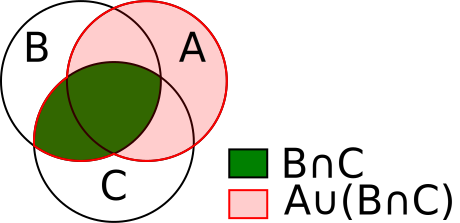
\includegraphics[width=0.4\textwidth]{img/Aunion_BintersectC.pdf} & 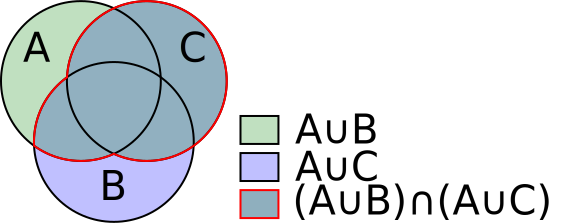
\includegraphics[width=0.4\textwidth]{img/AunionB_intersect_AunionC.pdf}
\end{tabular}
\end{center}
\end{myproof}
und die \underline{Absorbtionsgesetze}
\begin{equation}\forall a,b : A \cap (B \cup A) = A\end{equation}
\begin{equation}\forall a,b : A \cup (B \cap A) = A\end{equation}
Beweis analog.
\subsection{Komplement}
Im Folgenden sind die von uns betrachteten Mengen $A, B, C$... Teilmengen der \underline{Grundmenge G}.
$$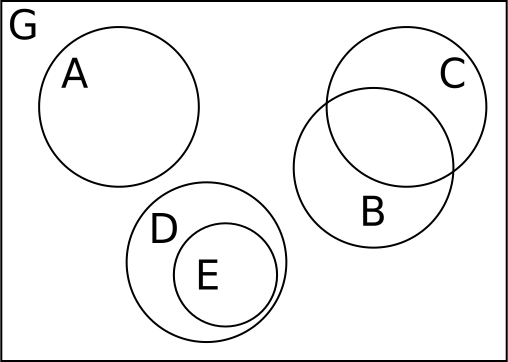
\includegraphics[width=0.4\textwidth]{img/underlying_set.pdf}$$
\begin{mydef}\begin{equation}\overline{A} := \{x \quad | \quad x \not \in A\}\end{equation} heisst Komplementärmenge (Komplement) der Menge $A$\end{mydef}
\begin{center}\includegraphics[scale=0.5]{img/Set_Komplement.png}\\$\overline{A}$ entspricht in diesem Bild $A^c$ in der Grundmenge $U$.\end{center}
%TODO: Besseres Bild?
Dann sehen wir, dass
\begin{equation}A \cap \overline{A} = \emptyset\end{equation}
und
\begin{equation}A \cup \overline{A} = G\end{equation}
Weiter gelten die \underline{Gesetze von De Morgan}:
\begin{equation}\overline{A \cap B} = \overline{A} \cup \overline{B}\end{equation}
\begin{equation}\overline{A \cup B} = \overline{A} \cap \overline{B}\end{equation}
\begin{myproof}Wir beweisen mit zwei Diagrammen:
\begin{center}\begin{tabular}{c c}
$\overline{A \cup B}$ & $\overline{A} \cap \overline{B}$\\
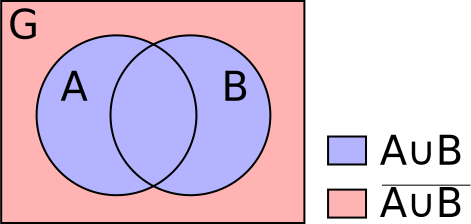
\includegraphics[width=0.4\textwidth]{img/AunionB_complement.pdf} & 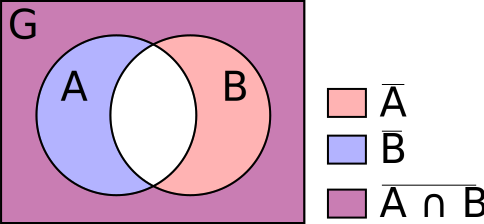
\includegraphics[width=0.4\textwidth]{img/Acompl_intersect_Bcompl.pdf}
%TODO: Zwei Diagramme (De Morgan)
\end{tabular}
\end{center}\end{myproof}
\subsection{Differenz}
\begin{center}\includegraphics[scale=0.5]{img/Set_Differenz.png}\end{center}
\begin{mydef}\begin{equation}A \setminus B = \{x \quad | \quad x \in A \land x \not \in B\}\end{equation}
heisst \underline{Differenz} der Mengen $A$ und $B$.\end{mydef}
Wir finden
\begin{equation}A \setminus B = A \cap \overline{B}\end{equation}
TODO %TODO: Bild zur obrigen Vereinfachung
\begin{equation}B \cap (C \setminus A) = (B \setminus A) \cap (C \setminus A)\end{equation}
Wir sagen, dass die Differenz \underline{rechtsdistributiv} bezüglich des Schnittes ist. Sie ist aber \underline{nicht linksdistributiv} des Schnittes.
\subsection{Symetrische Differenz}
\begin{center}\includegraphics[scale=0.5]{img/Set_SymDifferenz.png}\end{center}
\begin{mydef}\begin{equation}A \Delta B := (A \setminus B) \cup (B \setminus A)\end{equation}
heisst die \underline{symetrische Differenz} der Mengen $A$ und $B$.\end{mydef}
\section{Kartesisches Produkt}
Nach René Decartes, 1596 bis 1650, Paris, Stockholm
\begin{mydef}\begin{equation}A \times B := \{(x/y) \quad | \quad x \in A \land y \in B\}\end{equation}heisst \underline{kartesisches Produkt} der Mengen $A$ und $B$.\end{mydef}
Es ist also
\begin{equation}A \times B \neq B \times A\end{equation}
Wir sagen auch, dass $A \times B$ die Menge der geordneten Paare ist. Sind $A, B \in \mathbb{R}$, so können wir $A \times B$ im \underline{kartesischen Koordinatensystem} darstellen.
\begin{mydef}Für $n \in \mathbb{N}$ ist
\begin{equation}A^n := A \times A \times A \times ... \times A \quad \mbox{(n Faktoren)}\end{equation}\end{mydef}

\end{document}